\documentclass[a4paper,12pt]{article}

%Include Packages
\usepackage{amsmath}
\usepackage{amssymb}
\usepackage{textcomp}
\usepackage{graphicx}
%Fix margin issue
\usepackage[margin=0.8in]{geometry}
\usepackage{float}

\setcounter{tocdepth}{4}

%Top Matter
\title{Numerical Studies of Stochastic Spin Systems}
\author{Michael Conroy\\
  \\
  PHY 471 Capstone Project \\
  Spring 2014 \\
  Professor: Dr. Matthew Enjalran\\
  \date{}}

\begin{document}

\maketitle

\begin{abstract}
Analytic and numerical studies of stochastic spin systems were conducted to explore magnetic phase transitions. By applying the Monte Carlo Metropolis Algorithm (MCMA) to simulations of the classical Heisenberg Paramagnet in an external magnetic field, no phase transitions was found as expected of this non-interacting system. Conversly, MCMA simulations of the classical, isotropic, 3D Heisenberg Model explicitly show a second order phase transition at its critical temperature, $T_c \approx 1.45 K$. This is due to the cooperative effects of nearest neighbor interactions.
	

\end{abstract}
 
\pagebreak

%\tableofcontents
%\listoffigures
%\listoftables

\pagebreak

\section{Introduction}
A study of stochastic spin system was undertaken during the 2013-2014 school year for a PHY 499 Independent Study and PHY 471 Capstone Project. The fields of thermodynamics, statistical mechanics, and numerical methods were applied to compare analytic solutions to MCMA simulations of the classical Ising Paramagnet and the classical Heisenberg Paramagnet in an external magnetic field. Next, the 2D and 3D Ising Model were explored for periodic boundary conditions in preparation for simulating the classical, isotropic, 3D Heisenberg Model. The overall goal was finally met by comparing the Heisenberg Paramagnet with the critical phenomena demonstrated by the 3D Heisenberg Model.

Magnetism and magnetic systems in statistical physics provide a rich wealth of phenomena to study, especially that of critical phenomena near critical points in correlated systems. Several different thermodynamic properties such as specific heat, magnetization, and susceptibility exhibit critical behavior at critical points, and what is often visible is a sharp change in the properties of a substance. Of course, uncorrelated systems do not undergo a phase transition, but they do exhibit interesting magnetic behavior in external magnetic fields.

Comparing the correlated and uncorrelated systems illustrates the differences well. Phase transitions do not exist for non-interacting paramagnetic systems, because while paramagnets exhibit some magnetic properties in an external field, they do not show a macroscopic magnetization. The phase change such as that exhibited by the 3D Heisenberg Model exhibits a permanent macroscopic magnetization at an obvious critical point.

The studies in this paper illustrate paramagnetic magnetization of a classical Heisenberg Paramanget in an external magnetic field and the magnetic, second order phase transition of the 3D Heisenberg Model. No critical phenomena was found for the paramagnet, and a magnetic, second order phase transition was clearly evident at $\beta = 0.69$ for the 3D Heisenberg model as predicted in the literature. \cite{arxiv1, arxiv2} However, the susceptibility proved difficult to calculate.

%%%%%%%%%%%%%%%%%%%%%%%%%%%%%%%%%%%%%%%%%%%%%%%%%%%%%%%%%%%%%%%%%%%%
%%%%%%%%%%%%%%%%%%%%%%%%%%%%%%%%%%%%%%%%%%%%%%%%%%%%%%%%%%%%%%%%%%%%
%%%%%%%%%%%%%%%%%%%%%%%%%%%%%%%%%%%%%%%%%%%%%%%%%%%%%%%%%%%%%%%%%%%%

\section{Background and Theory}

\subsection{Statistical Mechanics}
The studied spin systems are characterized by the canonical ensemble. The probability of finding the model in any particular state is therefore proportional to the Boltzmann factor
\begin{equation}\label{eq:probability}
		P_\mu = \frac{1}{Z(\beta)}e^{-\beta E(\mu)}
\end{equation}
where $Z(\beta)$ is the partition function
	\begin{equation}\label{eq:partition}
		Z(\beta) = \sum_\mu e^{-\beta E(\mu)}
	\end{equation}
Most macroscopic thermodynamics variables of a system can be expressed by the partition function or its derivatives. The variables - energy, magnetization, susceptibility, heat capacity and absolute magnetization - are calculated, as well as the averages of those variables. The system's dependence on temperature is carried by the temperature's appearance in the probability term.

Exact solutions to the thermodynamic quantities for the Heisenberg Paramagnet were calculated and compared to MCMA simulations using the energy fluctuations form of the specific heat and magnetic fluctuations form of the susceptibility. For example, a comparison of the exact and fluctuations form of the specific heat per site:
	\begin{equation}\label{specific_heat_example}
		C =\frac{k\beta^2}{N}\frac{\partial^2\log{Z}}{\partial\beta^2} = \frac{k\beta^2}{N}(\left< E^2 \right> - \left< E \right>^2)
	\end{equation}
Since no exact solution exists for the 3D Heisenberg Model, only MCMA simulations were run using the fluctuations form of the specific heat and susceptibility. The energy and magnetization calculated in the simulations are averages over the lattice or site considered. \cite{gould}
\subsection{Magnetism and Magnetic Phase Transitions}
	\subsubsection{Para-, Ferro-, and Antiferromagnetism}
	Magnetically ordered solids separate broadly into many groups of magnetism, three of which we discuss here: ferromagnetism, antiferromagnetism, paramagnetism. In ferromagnets, the local moments are energetically preferred to be all aligned in a particular direction, the direction of spontaneous magnetization, so that the solid as a whole has a nonzero spontaneous magnetic moment. In antiferromagnets, adjacent local
moments prefer to be antialigned; paramagnets have zero spontaneous magnetization, because their moments are randomly oriented. 
	\begin{figure}[H]
		\centering
		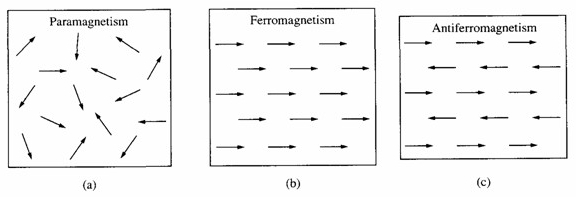
\includegraphics[scale=0.5]{ferro_para_anti}
		\caption{Schematic representations of magnetic dipole arrangements in (a) paramagnetic, (b) ferromagnetic, and (c) antiferromagnetic materials.}
		\label{fig:Types_of_Magnetism}
	\end{figure}
	\subsubsection{Magnetic Phase Transitions}
	The generatlized Hamiltonian of concern is
	\begin{equation}\label{eq:full_hamiltonian}
			H = -J\sum_{<ij>}\vec{S_i}\cdot\vec{S_j} + B\sum_i{\vec{S_i}}.
		\end{equation}
The first term is the exchange interaction and is responsible for the cooperative behavior and the possibility of a phase transition. J is the exchange energy (strength of the interaction): positive favors parallel and negative anti-parallel alignment of the spins. This term is relevant for the exploration of the 3D Heisenberg Model, where the external magnetic field $B = 0$.

The second term is the Zeeman interaction and responsible for the magnetic behavior of spins in a non-zero magnetic field. Therefore, the only influence ordering the spins is the magnetic field. In the case of the classical Ising and Heisenberg Paramgnets discussed here, $J = 0$, they do not interact, there are no cooperative effects, and hence no phase transition.

While the paramagnets display no magnetic phase transition, the 3D Heisenberg Model demonstrates a second order ferromagnetic phase transition. At a certain temperature, the critical temperature or critical point, the disordered paramagnetic Heisenberg system changes from one displaying seemingly no macroscopic magnetization into a spontaneously magnetized system -- a ferromagnetic system. The phase transition comes about purely from the cooperative behavior of the spins due to the exchange interaction.

Second order phase transitions occur when a new state of reduced symmetry develops continuously from the disordered high temperature phase. The ordered phase has a lower symmetry than the Hamiltonian -- the phenomenon of spontaneously broken symmetry. There will therefore be a number (sometimes infinite) of equivalent (e.g. equal free energy) symmetry related states. These are macroscopically different, and so thermal fluctuations will not connect one to another in the thermodynamic limit. To describe the ordered state we introduce a macroscopic order parameter that describes the character and strength of the broken symmetry.

When the phase transition is happening between an ordered and a disordered phase, it is possible to construct an order parameter compatible with the symmetries of the system, vanishing in the disordered phase while being finite in the ordered phase. Although for a ferromagnetic-paramagnetic transition the choice of this order parameter is usually obvious (i.e. the magnetization), there are also systems with hidden order, where the nature of the order parameter is unknown. It is possible to define the correlation function of the order parameter. Far away from a phase transition, the correlations decay usually exponentially, defining characteristic length and time scale, $\xi$ and $\tau$, respectively. \cite{landau, newman}

At second order transitions, the order parameter vanishes continuously at $T = T_c$, when increasing the temperature. Usually, there exists an upper critical dimension $d_c$ for a given phase transition, so that the fluctuations do not play an essential role and mean field approximations. For example, the Ising Model exhibits a phase transition when $d_c \geq 2$, and the Heisenberg model exhibits a phase transition when $d_c \geq 3$. At these dimensions, the parameter fluctuations become very important.

Spontaneous breaking of symmetry is also an important signature of a phase
transition: the disordered phase typically exhibits the symmetries of the microscopic model. This manifests also in the vicinity of the global minimum of the thermodynamic potential, which usually also has large symmetry in the disordered phase. The second order transition shifts the global minimum in a direction chosen spontaneously to a point of reduced symmetry in parameter space. \cite{dissertation}

%%%%%%%%%%%%%%%%%%%%%%%%%%%%%%%%%%%%%%%%%%%%%%%%%%%%%%%%%%%%%%%%%%%%
%%%%%%%%%%%%%%%%%%%%%%%%%%%%%%%%%%%%%%%%%%%%%%%%%%%%%%%%%%%%%%%%%%%%
%%%%%%%%%%%%%%%%%%%%%%%%%%%%%%%%%%%%%%%%%%%%%%%%%%%%%%%%%%%%%%%%%%%%

\section{Models and Methods}

\subsection{The Magnetic Models}
	\subsubsection{The Classical Paramagnet}
	The classical paramagnet is expressed by the Hamiltonian
	\begin{equation}\label{eq:zeeman}
		H = -\sum_{i=1}^N{\vec{b}\cdot\vec{S_i}},
	\end{equation}
	which is a simplified version of the Zeeman interaction. This is the sum over all sites of the dot product of the effective magnetic field $\vec{b}$ along the z-axis and each site's spin, $\vec{S_i}$. The Heisenberg Paramagnet is a continuous spin model, so $\vec{S_i} = (\sin\theta_i\cos\phi_i, \sin\theta_i\sin\phi_i, \cos\theta_i)$, where $|\vec{S_i}| = 1$.  From these equations, the Hamiltonian for the Heisenberg Paramagnet will be derived. The average magnetization per site MCMA simulation and susceptibility were not calculated.
	\subsubsection{The Heisenberg Paramagnet}
	\begin{figure}[H]
			\centering
			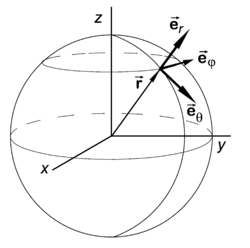
\includegraphics[scale=5.0]{spherical_unit_vector}
			\caption{Spherical unit vector of a Heisenberg spin.}
			\label{fig:spherical_unit_vector}
		\end{figure}
		\paragraph{Description and Analytic Solution}
		The classical Heisenberg Paramagnet spin at each site is defined by two sphereical polar angles, but if the $\vec{b}$ direction is defined as the global $z$-direction, then the Zeeman interaction of \eqref{eq:zeeman} becomes
		\begin{equation}\label{eq:heisenberg_PM_hamiltonian}
			H = -b\sum_{i=1}^N{\cos \theta_i},
		\end{equation}
		because the energy of the spin is only dependent on the polar angle $\theta_i$. The partition function for a system of $N$ independent spins in an external magnetic field is then
		\begin{equation}\label{eq:heisenberg_para_partition_fxn}
			Z_N = \left[\frac{4\pi}{\beta b}\sinh(\beta b)\right]^N = (Z_1)^N,
		\end{equation}
		and the partition function for one spin is $Z_1 = (4\pi/\beta b)\sinh(\beta b)$. Again, all thermodynamic quantities for this model are now analytically calculable.
		\paragraph{MCMA Solution Form}
		For the classical Heisenberg Paramagnet model, the average energy per site $\langle E \rangle$, the specific heat $C$, and the average magnetization per site $\langle M \rangle$ are (let $k = b = 1$ here):
		\begin{equation}\label{eq:heisenberg_PM_avg_energy}
			\frac{\langle E \rangle}{N} = -\frac{1}{N}\sum_j^N{\cos \theta_j},
		\end{equation}
		\begin{equation}\label{eq:heisenberg_PM_specific_heat}
			C = \frac{\beta^2}{N}(\left< E^2 \right> - \left< E \right>^2),
		\end{equation}
		and
		\begin{equation}\label{eq:heisenberg_PM_avg_magentization}
			m = \frac{\langle M \rangle}{N} = -\frac{1}{N}\left|\sum_j^N{\cos \theta_j}\right|.
		\end{equation}
		
	\subsubsection{Heisenberg Model}
			\begin{figure}[H]
			\centering
			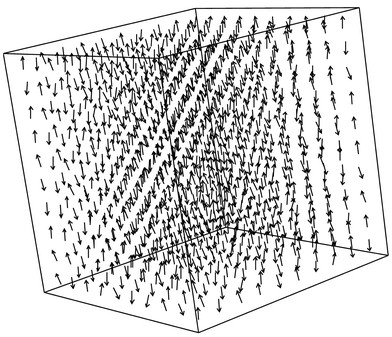
\includegraphics[scale=0.5]{lattice}
			\caption{Paramagnetic ($T>T_c$) Heisenberg Model on a 10x10x10 Lattice.}
			\label{fig:heisenberg_lattice}
		\end{figure}
		\paragraph{Description}
The classical, isotropic, 3D Heisenberg Model on the simple cubic lattice is now considered. The spins themselves are considered in the same manner as the Heisenberg Paramagnet, but now cooperative effects are applied by setting $B = 0$ and $J = 1$ for the ferromagnetic case. The zero-field version of the model was chosen for simplicity as is usually the case for multi-dimensional spin models with interacting spins.	\cite{scribd}

Easy to state and widely applicable, the Heisenberg Model is also extremely difficult to analyze.The Heisenberg model is considered the superior to the Ising model in the case of magnetic systems, but its basis on more complicated interactions between spins makes it mathematically complex. On the other hand, the Ising model, derived from statistical physics, is much simpler and much more popular. However, the Heisenberg Model was chosen for its better approximation of physical reality.
		\paragraph{MCMA Solution Form}
The average energy per site $\langle E \rangle$, the $rms$ magnetization  $\langle M \rangle$, the specific heat $C$, and the magnetic susceptibility $\chi$ are (let $k = b = 1$ here)
	\begin{equation}
		\frac{\langle E \rangle}{N} = -\frac{J}{2N}\sum_{<ij>}^{N}\vec{S_i}\cdot\vec{S_j},
	\end{equation}
	(factor of $\frac{1}{2}$ for double counting)
	\begin{equation}
		C = k\beta^2(\left< E^2 \right> - \left< E \right>^2),
	\end{equation}
	and
	\begin{equation}
		m_{rms} = \sqrt{M_x^2 + M_y^2 + M_z^2},
	\end{equation}
	where $\displaystyle M_\alpha = \frac{1}{N}\sum_i{\vec{S_{i\alpha}}}$.

The Heisenberg system has an order parameter with multiple components and all the three components are equally important. The order parameter is invariant under global rotation and therefore we need to keep track of its magnitude alone. However, this causes an issue calculating the magnetic susceptibility, $\chi$. Thus, the standard form of $\chi$
			\begin{equation}
				\chi = \frac{\beta}{N}(\langle M^2 \rangle - \langle M \rangle^2) = \beta N(\langle m^2 \rangle - \langle m \rangle^2)
			\end{equation}	
cannot be used, and the correlation function must be computed. This step was not completed for this paper due to time constraints and the inherent complexity involved with implementing the calculation.		     	  	

\subsection{The Metropolis Monte Carlo Method}
	\subsubsection{Introduction}
	The field of numerical analysis is applied to intractable problems and problems without analytic solutions such as the $d \geq 3$ dimensional Ising Model and 3D Heisenberg Model. The MCMA method was utilized for the models explored in this paper. The uniform pseudo-random number generators built in to Fortran and C were used and consistently seeded to maintain random number generation among simulations written in each language.
	\subsubsection{Implementation}
A standard MCMA method was applied. The Metropolis Algorithm importance sampling was implemented. The MCMA importance sampling algorithm is now described step-by-step:
	\begin{enumerate}
		\item Choose initial state
		\item Choose a site
		\item Calculate $\Delta E$ if ``flip" the spin
		\item If $\Delta E \le 0$, accept ``flip" and go to (7), otherwise (5)
		\item RNG: $0 < r < 1$
		\item If $r < \exp(-\beta \Delta E)$, accept ``flip"
		\item Go to next site and go to (3)...
	\end{enumerate}
The spin ``flip" corresponds to choosing new, randomly generated $\theta$ and $\phi$ angle for the Heisenberg Paramagnet and 3D Heisenberg Model spins. \cite{landau}

%%%%%%%%%%%%%%%%%%%%%%%%%%%%%%%%%%%%%%%%%%%%%%%%%%%%%%%%%%%%%%%%%%%%
%%%%%%%%%%%%%%%%%%%%%%%%%%%%%%%%%%%%%%%%%%%%%%%%%%%%%%%%%%%%%%%%%%%%
%%%%%%%%%%%%%%%%%%%%%%%%%%%%%%%%%%%%%%%%%%%%%%%%%%%%%%%%%%%%%%%%%%%%

\section{Results and Discussion}
\subsection{Heisenberg Paramagnet}
	\begin{figure}[H]
			\centering
			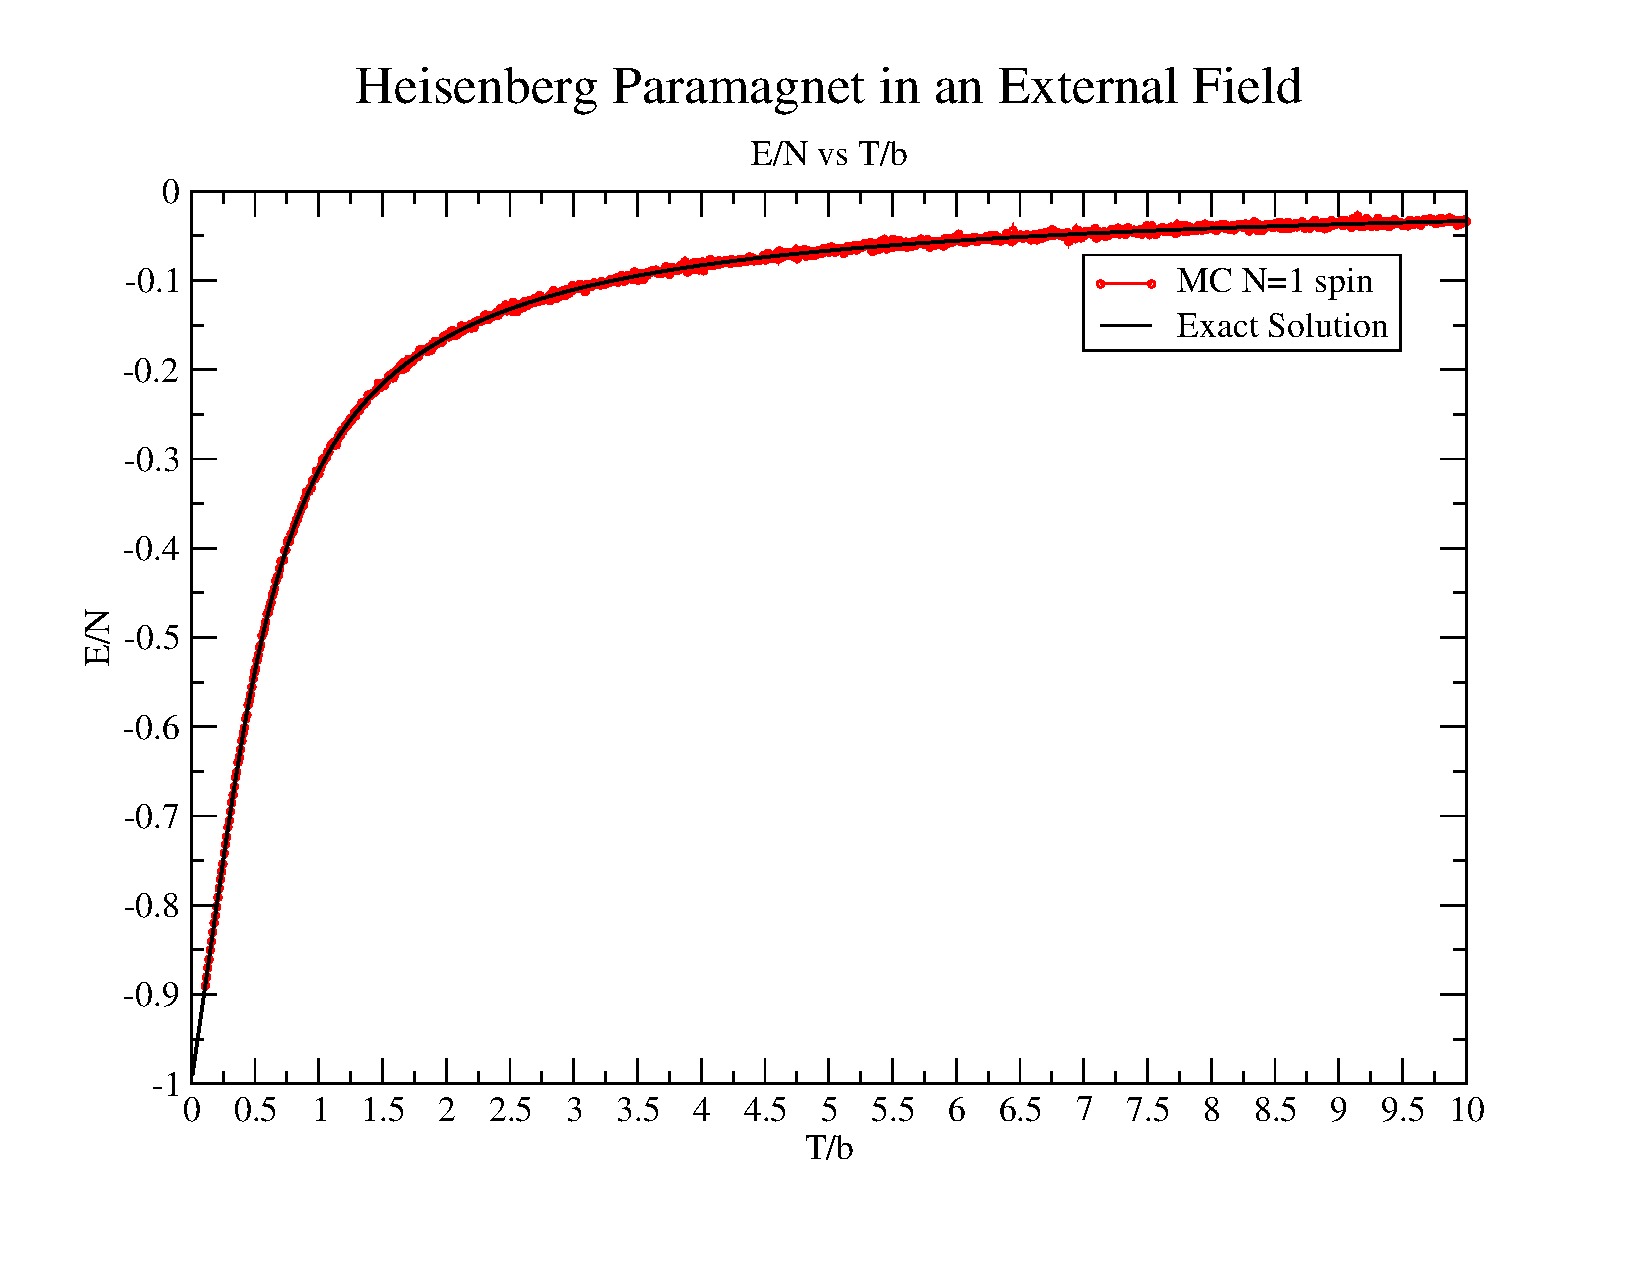
\includegraphics[scale=0.65]{e_n.pdf}
			\caption{Average energy per site for the Heisenberg Paramagnet.}
			\label{fig:heisenberg_PM_e_avg}
		\end{figure}
		
		The average energy per site MCMA simulation agrees with the exact solution. As the spins align with the external magnetic field, the energy reduces to the lowest level $\langle E \rangle = -1$.
		
		\begin{figure}[H]
			\centering
			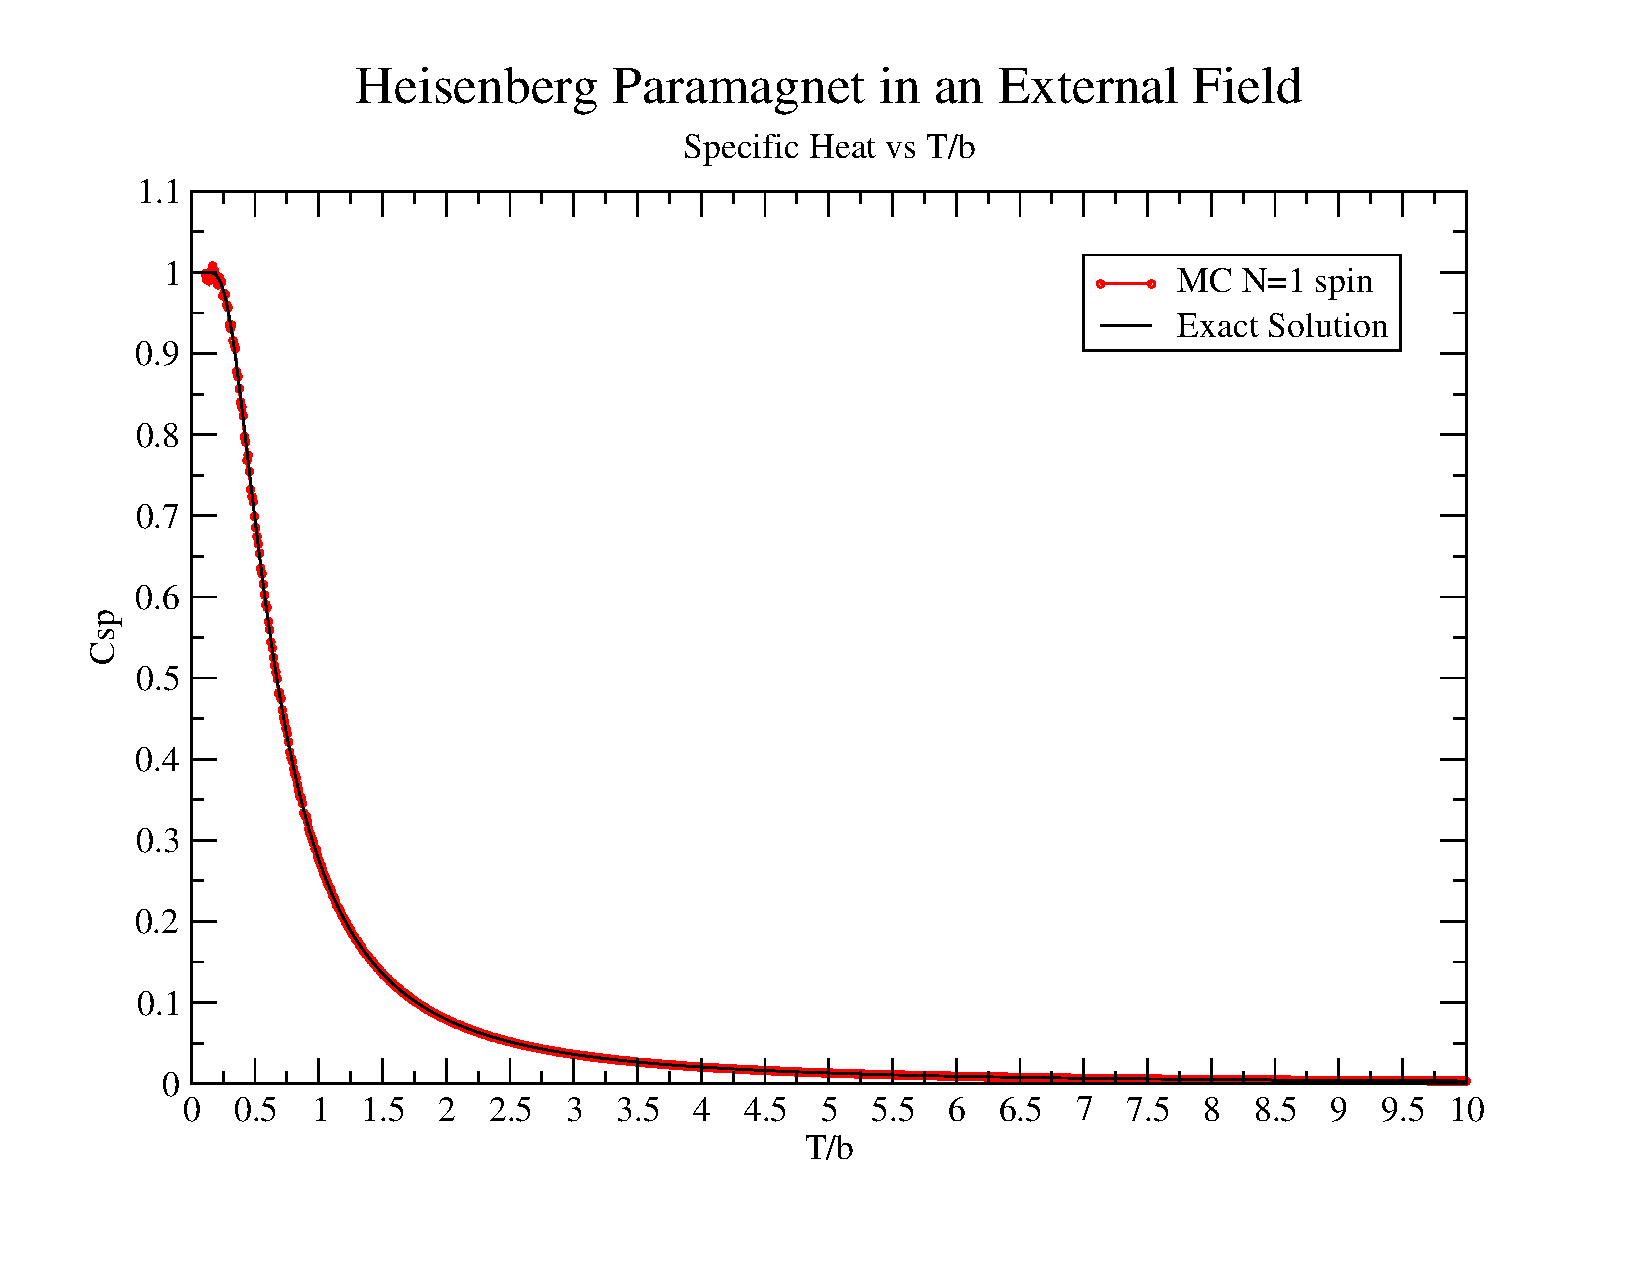
\includegraphics[scale=0.65]{sp.pdf}
			\caption{Specific heat for the Heisenberg Paramagnet.}
			\label{fig:heisenberg_PM_sh}
		\end{figure}
		
		The specific heat is indicated of the fluctuations that take place as the energy curves down and the spins align with the magnetic field. The clumping of the MCMA solution points at the top of the curve is due to critical slowing down because of the Metropolis Algorithm's issues at the critical point. There is no evidence here of a phase transition, because the lowest energy state and maximum fluctuations exist at $T = 0 K$ where the specific heat is greatest.
		
		\begin{figure}[H]
			\centering
			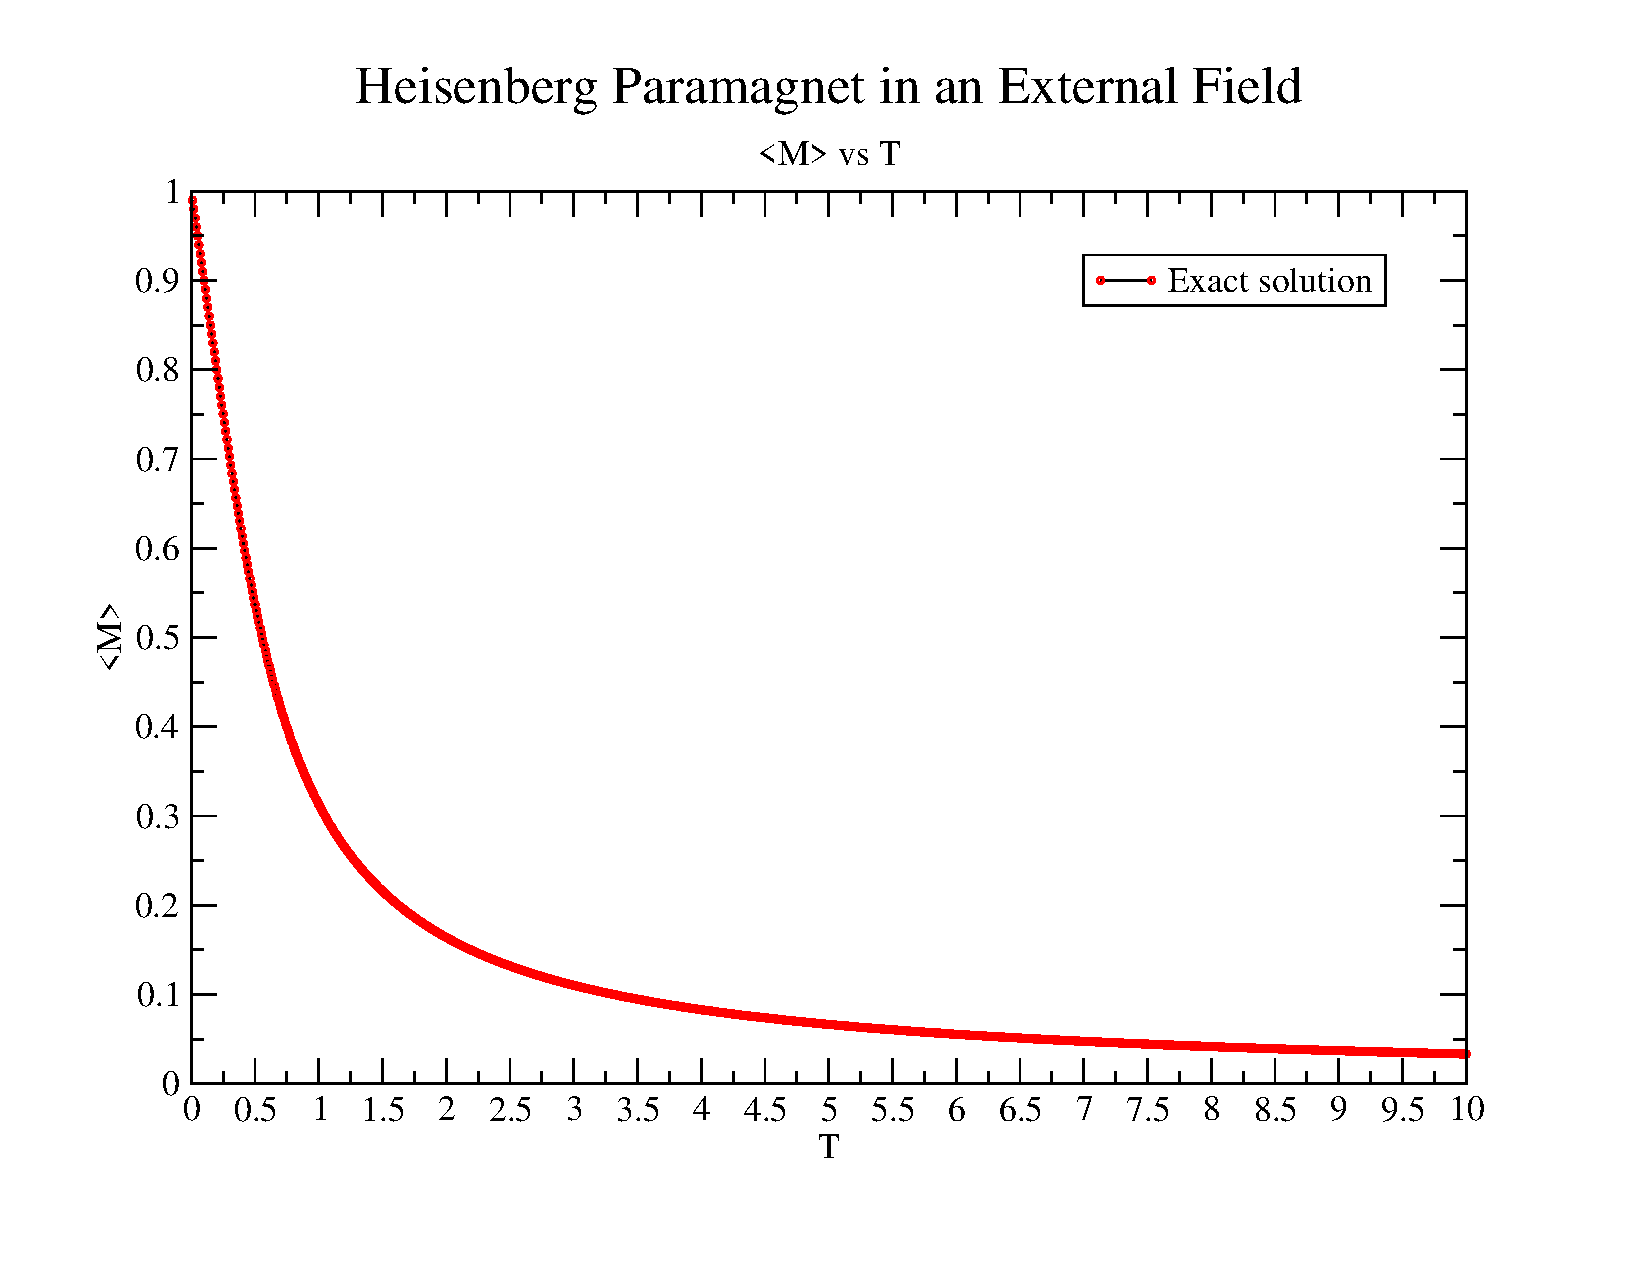
\includegraphics[scale=0.65]{m_avg_PM.pdf}
			\caption{Average magnetization exact solution for the Heisenberg Paramagnet.}
			\label{fig:heisenberg_PM_m_avg}
		\end{figure}
		
		The average magnetization exact solution shows a peak of $\langle M \rangle = 1$ at $T = 0 K$. As expected, maximum magnetization is indicative of spin abd magnetic field alignment. There is no continuous change from zero-magnetization to a non-zero magnetization across a critical point, only a trend towards a maximum magnetization as the system cools towards $T = 0 K$. Therefore, no phase transition is evident.

\subsection{Heisenberg Model}
	\begin{figure}[H]
			\centering
			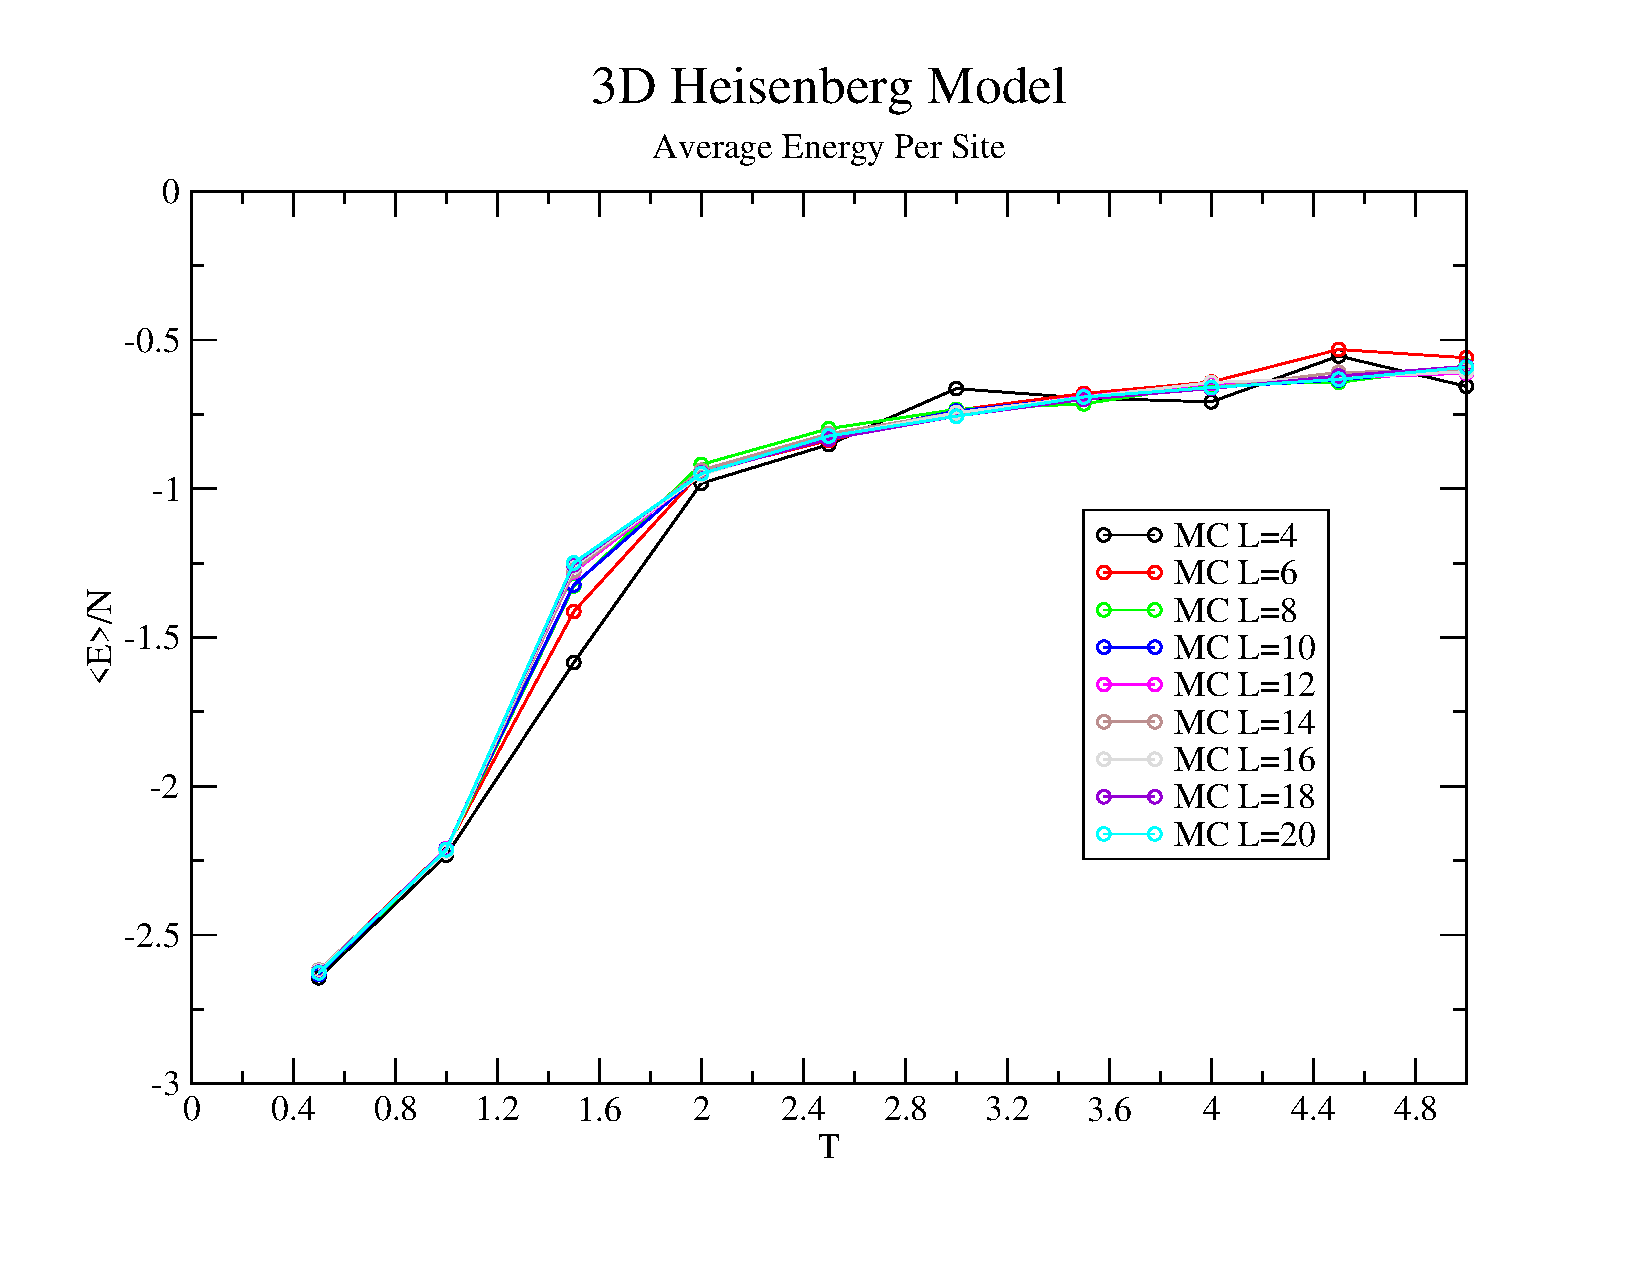
\includegraphics[scale=0.65]{e_avg.pdf}
			\caption{Average energy per site for the 3D Heisenberg Model.}
			\label{fig:heisenberg_e_avg}
		\end{figure}
		
		The average anergy per site agrees well with expectations. The energy will trend to a minimum of $\langle E \rangle = -3$ after curving down at $T_c \approx 1.45 K$ when the spins align at the lowest energy potential. In the thermodynamic limit, the energy should trend to $\langle E \rangle = 0$, but this simulation maxes out at $T = 5 K$. A larger temperature range will show the trend towards zero. Finite size effects are evident in the steepening of the curve around the critical temperature as the lattice sizes increase. In the thermodynamic limit, the graph should curve straight down at the critical temperature.

		\begin{figure}[H]
			\centering
			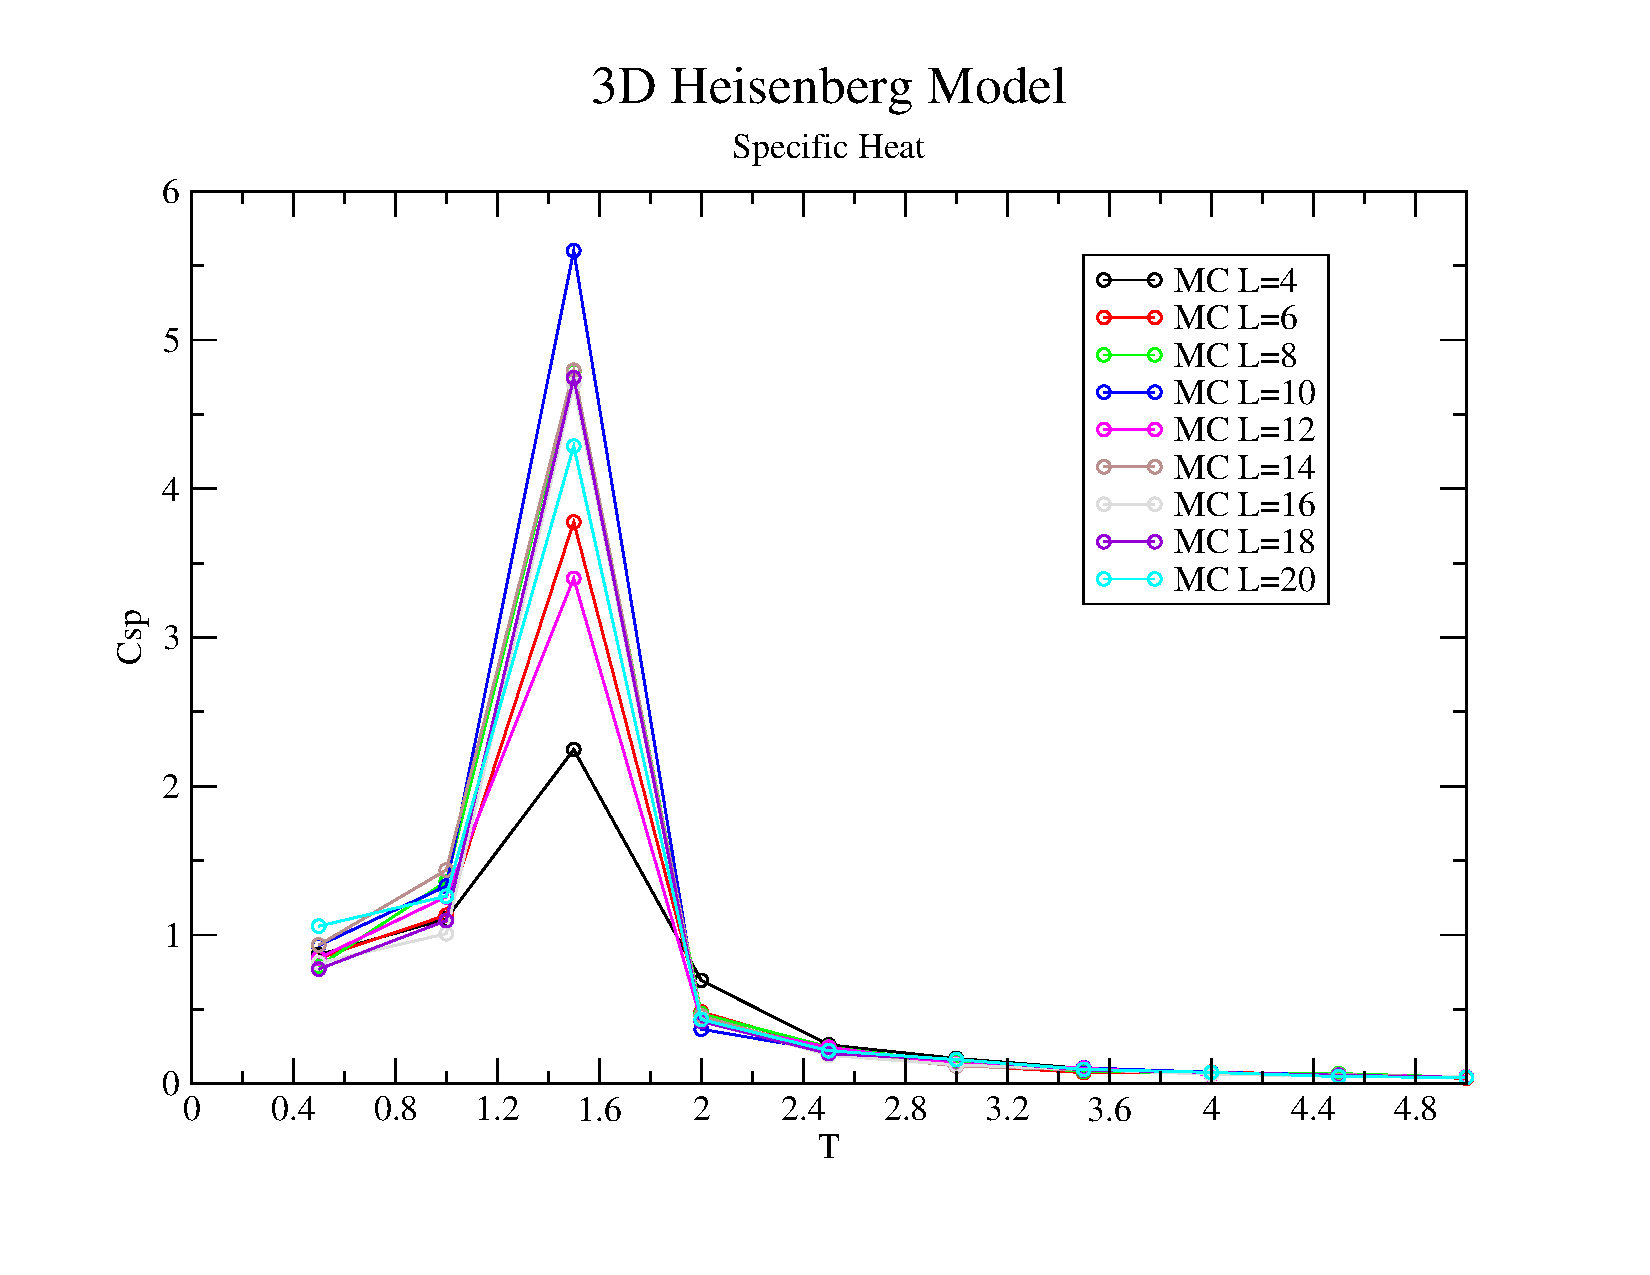
\includegraphics[scale=0.65]{cplot}
			\caption{Heat capacity for the 3D Heisenberg Model.}
			\label{fig:heisenberg_heat_capacity}
		\end{figure}
		
		The heat capacity curve also agrees well with expectations. The peak should trend to infinity and width should trend to zero at the critical temperature in the thermodynamic limit. The data clearly details this as lattice sizes grow from $L = 4$ to $L = 10$. For larger lattice sizes, the peak should grow and narrow even more, but critical slowing down issues with the Metropolis Algorithm implementation clearly demonstrate that the higher lattice dimension simulations were not run long enough at the critical point. This also implies that the higher lattice sizes may not have relaxed enough thermodynamically and increased equilibration and measurement phase runs are required.

		The non-zero magnitude of the specific heat under the critical temperature is important to note. The 3D Heisenberg Model has a continuum of ground states. Therefore, fluctuations will still occur when the spins are aligned, but the entire system will randomly reorient itself in any direction. The spins will stay aligned, but the direction they point will randomly fluctuate.
		
		\begin{figure}[H]
			\centering
			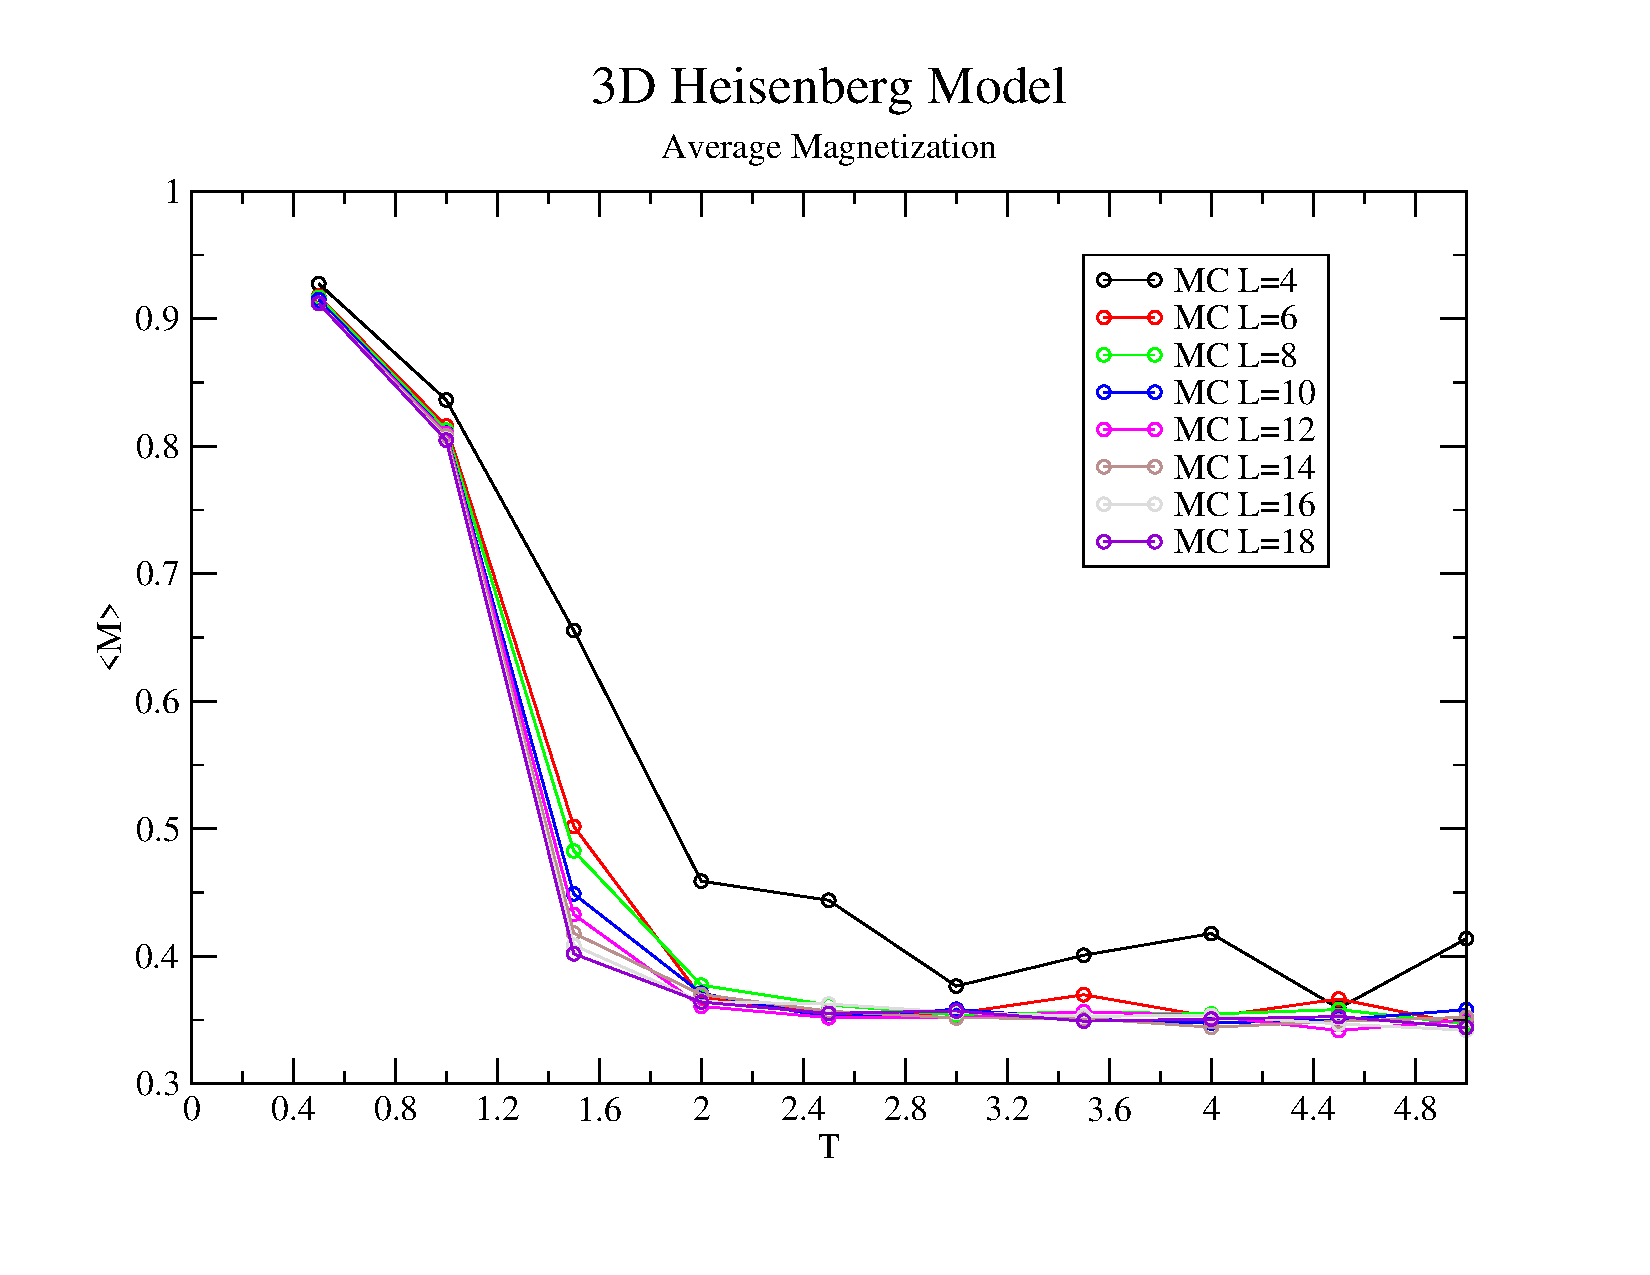
\includegraphics[scale=0.65]{m_avg}
			\caption{Average magnetization per site for the 3D Heisenberg Model.}
			\label{fig:heisenberg_m_avg}
		\end{figure}

		The magnetization demonstrates the same steepening at the critical point. The curve also doesn't trend towards zero in the thermodynamic limit, but not due to the chosen temperature range. The magnitude of the magnetization is considered, not the magnetization itself, so the fluctuations will always cause a positive magnetization--an overestimation. This is a direct result of calculating $m_{rms}$ and is expected.
		
		Clearly, a continuous phase transition occurs. A zero magnetization region, $T > T_c$, is separated from a non-zero magnetization region, $T < T_c$, around a critical point where the magnetization rises and susceptibility diverges. The order parameter defines as the magnetization for this model demonstrates  a clear ferromagnetic phase change at $T_c = 1.45 K$.

%%%%%%%%%%%%%%%%%%%%%%%%%%%%%%%%%%%%%%%%%%%%%%%%%%%%%%%%%%%%%%%%%%%%
%%%%%%%%%%%%%%%%%%%%%%%%%%%%%%%%%%%%%%%%%%%%%%%%%%%%%%%%%%%%%%%%%%%%
%%%%%%%%%%%%%%%%%%%%%%%%%%%%%%%%%%%%%%%%%%%%%%%%%%%%%%%%%%%%%%%%%%%%

\section{Conclusion}
The data matches expectations and the predictions from iterature. Magnetic behavior was shown for the Heisenberg Paramagnet, which lacked a magnetic phase change as expected. Agreeing with the literature quite well, a phase transition at the critical temperature of $T_c \approx 1.45 K$ was evidenced for the classical, isotropic, 3D Heisenberg Model.

Three issues remain. The first is how the the magnetic susceptibility of the 3D Heisenberg Model was not as straightforward to calculate as assumed. The second concern is an acceptance ratio oddity for this model's simulation where artificially high ratios do not correlate well with how the model was programmed. Instead of slightly perturbing the $\theta$ and $\phi$ angles at each MCMA update, a new, completely random angle was chosen for both. Therefore, the acceptance ratios should be small instead of on the order of $\approx0.80$ at the start of each simulation to $\approx0.50$ at the conclusion.

The final concern is how the 3D Heisenberg Model was programmed. The larger simulations took on the order of a week and a half to run, but critical slowing down still became evident. The larger simulations were therefore not run for long enough times to let the system fully relax before measurements were taken. Three and four dimensional pseudo-arrays were implemented in C, which caused extremely slow run times. Altering the code to run more efficiently with one and two dimensional arrays and implementing structures would allow for shorter run times, and therefore increased runs for the equilibration and measurement phases.
    
%%%%%%%%%%%%%%%%%%%%%%%%%%%%%%%%%%%%%%%%%%%%%%%%%%%%%%%%%%%%%%%%%%%%
%%%%%%%%%%%%%%%%%%%%%%%%%%%%%%%%%%%%%%%%%%%%%%%%%%%%%%%%%%%%%%%%%%%%
%%%%%%%%%%%%%%%%%%%%%%%%%%%%%%%%%%%%%%%%%%%%%%%%%%%%%%%%%%%%%%%%%%%%

\section{Acknowledgments}
The author would like to thank Tom Sadowski for his invaluable help with programming multidimensional arrays with pointers in C.

%%%%%%%%%%%%%%%%%%%%%%%%%%%%%%%%%%%%%%%%%%%%%%%%%%%%%%%%%%%%%%%%%%%%
%%%%%%%%%%%%%%%%%%%%%%%%%%%%%%%%%%%%%%%%%%%%%%%%%%%%%%%%%%%%%%%%%%%%
%%%%%%%%%%%%%%%%%%%%%%%%%%%%%%%%%%%%%%%%%%%%%%%%%%%%%%%%%%%%%%%%%%%%

\begin{thebibliography}{9}
  
  \bibitem{arxiv1}
  {\tt arXiv:hep-lat/9301002}
  
  \bibitem{arxiv2}
  {\tt arXiv:hep-lat/9209017}
  
  \bibitem{gould}
  Gould, H., \& Tobochnik, J. (2010).
  \emph{Statistical and thermal physics: with computer applications}.
  Princeton, N.J.: Princeton University Press.
  

	\bibitem{landau}
  Landau, D. P., \& Binder, K. (2009).
  \emph{A guide to Monte Carlo simulations in statistical physics (3rd ed.)}.
  Cambridge: Cambridge University Press.
  
  \bibitem{newman}
  Newman, M. E., \& Barkema, G. T. (1999).
  \emph{Monte Carlo methods in statistical physics}.
  Oxford: Clarendon Press.
  \bibitem{dissertation}
  Rapp, \'Akos.
  \emph{Quantum Phase Transitions in Correlated Systems}.
  http://dept.phy.bme.hu/phd/dissertations/rapp\_dissertation.pdf
  
  \bibitem{scribd}
  Tangirala, Sairam.
  \emph{Monte Carlo Simulation of 1D Heisenberg Model}.
  http://www.scribd.com/doc/50664110/Monte-Carlo-Simulation-of-1D-Heisenberg-Model
  

\end{thebibliography}

\end{document}
